% Name: My Exercise Paper on Lott and Mustard (1997) v2_7
% Author: Yu Xia (Based on Dr. Scott Cunningham's materials)
% Description: The first version after Dr. Zervou's 2nd feedback (thanks to SOP), and after UT Writing Center's appointment (Mainly focusing on Abstract). Having checked grammar after v2_5. Clarify TWFE and DID according to Dr Hounghton
% Last Updated: Dec 11, 2022

\documentclass{article}

\usepackage{titlesec}

\usepackage{amsmath}
\usepackage{amssymb}

\usepackage{booktabs}
\usepackage{float}
\usepackage{colortbl}
\usepackage{xcolor}

\usepackage{a4wide}
\usepackage{setspace}
\usepackage{geometry}
\usepackage{parskip}

\usepackage{multirow}
\usepackage{adjustbox}
\usepackage{graphicx}
\graphicspath{ {../figures/} }

\usepackage[style=apa,backend=biber]{biblatex}
\addbibresource{samplebib.bib}

\usepackage{hyperref}
\hypersetup{
    colorlinks=true,
    linkcolor=black,
    urlcolor=blue
}

\DeclareRobustCommand{\bbone}{\text{\usefont{U}{bbold}{m}{n}1}}

\DeclareMathOperator{\EX}{\mathbb{E}}

\author{Yu Xia}
\title{``More Guns, Less Crime" Reexamine \\ \large An Approach of New DID Methods}
\date{Fall 2022}

\begin{document}
\maketitle

\nocite{*}

    State governments across the US began to implement the Right-To-Carry laws (RTC) in the 1980s. Different from the situation where only those people who were fully trusted by the governments were permitted to carry concealed weapons, the RTC removes some restrictions, granting permissions to any person as long as they satisfy certain criteria. The effect of the laws, along with the method to estimate it, have been widely discussed. The possible positive effect on crime is that the more armed criminals, the more chances to commit crime. But the RTC may also lead to the deterrence effect: victims have more guns as well. The increasing risk of being shot deters felons, leads to higher cost to commit crime, thus reducing the crime rate. Based on the state-level panel data between 1970 and 1992, this analysis reexamines the multi-period treatment effect of the RTC, for 7 categories of crime rates: Murder, Rape, Aggravated Assault, Robbery, Burglary, Auto Theft and Larceny. The first part of this research tries to replicate Lott and Mustard's research (1997) by the Two Way Fixed Effect (TWFE). Their research argues that the deterrence effect dominates. However, using TWFE has to satisfy some strict assumptions: parallel trends, no anticipation effect, homogeneity on both treatment effect and trends. Otherwise, the results of TWFE may be biased, even flip the sign. To compare with the TWFE, this reexamination also uses Callaway \& Sant'Anna's (2021) and Sun \& Abraham's (2021) methods to estimate Difference-in-difference (DID). Callaway \& Sant'Anna (2021) generate an overall ATT estimator. Different from the TWFE method, it only checks periods when there exists never-treated or not-yet-treated units. Sun \& Abraham's method (2021) reorganizes cohorts by relative periods before or after the treatment happens for a certain amount of time, and estimates by comparing cohorts. Using the traditional TWFE, the results in this analysis shows that these laws decrease murder and aggravated assault by 8.7\% and 7.8\% in the 10\% and 5\% significant level respectively, but they also increase auto theft by 8.2\%, significant at the 5\% level, and increase larceny by 4.4\%, significant at the 1\% level. On the contrary, by the results of Callaway \& Sant'Anna's method, murder decreases about 16.72\%, rape goes down by 1.46\%, aggravated assault is reduced by 5.7\%, robbery declined by 1.38\%, auto theft diminished 6.52\%, and larceny represents a 0.67\% reduction, only a less than 1\% increment for the burglary. More importantly, the RTC has insignificant impacts for all 7 categories. In the event study, the Sun \& Abraham method implies that the impact of RTC is only obvious around 5 years after this law was implemented. Most of the pre-trends for categories of crime fit in 95\% confidence intervals, but the post-trends are still insignificant. These results are similar to Aneja, Donohue and Zhang (2011), with even more insignificant influence on the RTC. By reexamining previous results of gun control, this research implies that the TWFE method is only convincing if the underlying assumptions are satisfied, and the DID methods show that RTC doesn't have a significant effect on crime rates.

\newpage

\begin{abstract}
    This research measures the causal effect of the RTC laws on 7 categories of crime across the United States. Based on the state-level data from 1970 to 1992, it discusses TWFE regression, and uses Callaway \& Sant'Anna's (2021) and Sun \& Abraham's (2021) DID methods. Even though the biased TWFE shows significant impact on crime, results of Callaway \& Sant'Anna's (2021) method implies that the impact of RTC on 6 of the 7 categories are negative. Sun \& Abraham's method implies that the impact of RTC is only obvious around 5 years after this law was implemented. Moreover, both DID methods show that the impact of the RTC laws have no significant effect on crime. 
\end{abstract}

\section{Introduction}

Around the 1980s, states in the U.S. began to implement Right To Carry Laws (also called ``RTC laws", ``shall-issue laws"), remarking a change in gun control laws. The effect of the RTC laws on crime, and its estimation, however, is controversial. This paper replicates Lott and Mustard's paper (1997) at first. They used TWFE to estimate the effect of these laws. Rather than focusing on county level data, this analysis uses state level data. Different from most previous works, this paper then reanalyzes this topic by 2 Difference-in-difference (DID) methods suggested by Callaway \& Sant'Anna (2021) and Sun \& Abraham (2021). By discussing the result, this paper might be helpful in providing some ideas about how to analyze the effect of RTC laws in different treatment times, and the effect of gun control policies. 

\section{Background and Economic Theory}

Under the policies before the 1980s, governments only grant licenses to citizens who could convince governments of their need for weapons. The RTC laws grant any citizens, who meet specified criteria, a permission to carry concealed weapons. Table 1 shows the states and the time of implementing these laws. This table only describes the situation before 1992, as Lott and Mustard's research (1997) did. 

\input{../tables/Table_1.tex}

Earlier works have discussed the effect of gun control laws. Kleck and Patterson (1993) used 2SLS to measure gun prevalence levels and city violence rates, and indicated that most gun control restrictions have no effect on both of them, with possible exceptions for moderate, popular and inexpensive controls. McDowall, David and Loftin (1995) examined the frequency of homicides in some urban areas, and found that murder increases. Though they admitted that the result differs from states, it's unlikely that their analysis supports the evidence of decreasing murder. Lott and Mustard's paper (1997) set off a wider discussion about the ``More gun, less crime" theory. Their work talked about whether the RTC laws could deter any categories of crime behaviors. The implementation of the RTC laws were set as a dummy variable in Lott and Mustard's paper (1997), and they used county-level data. If a county starts to implement these laws, the dummy variable will be set to equal 1. The intuition behind their theory is that, by allowing people to carry concealed weapons, felons might be more afraid of armed victims than before (sometimes, even become more afraid of victims than police). Thus the cost of crime increases, and felons are more unwilling to commit crime. The original paper tried to prove this intuition using the TWFE method, which is potentially problematic. According to the Lott and Mustard paper (1997), they found evidence that the implementation of the RTC laws has a significant effect on deterring felons behavior. Nevertheless, based on Lott and Mustard's model (1997), Black and Nagin (1998) argued that there is no detectable impact of the RTC laws. Ludwig (1998) exploited the minimum age requirements and concluded that shall-issue laws increase adult homicide rate. Ayres and Donohue (2003) pointed out the selection effect problem in Lott and Mustard's paper (1997), arguing that their conclusion is unreliable because of the discredited jurisdictional aggregation assumption and coding errors. Donohue and Ayres (2009) suggested that the RTC laws at the very least increase aggravated assault. Aneja, Donohue and Zhang (2011) tried to reanalyze Lott and Mustard's work (1997) and introduce the hybrid model, but found no significant evidence for the RTC laws helpful for decreasing crime. On the other hand, Moody and Marvell (2008, 2009) insisted that even though there was an initial increase in crime, crime decreases over time. But Donohue and Ayres (2009) claimed that researchers should be cautious about extending the time span. Using four methods discussed by Ayres and Donohue (2003), Plassmann and Whitley (2003) found annual reductions in murder rates.

The TWFE method, which is frequently used in Difference-in-difference (DID), however, has flaws as well. Goodman-Bacon (2021) decomposed the ``DD estimator", clarifying the hidden assumptions and restrictions in using TWFE. To fix the problem of TWFE, Callaway \& Sant'Anna (2021) and Sun \& Abraham (2021) introduced new estimators respectively. This paper will talk about their basic idea later.

\section{Data}

The data comes from Aneja, Donohue and Zhang (2011)'s work which tries to replicate Lott and Mustard (1997). Instead of using the county-level data which has substantial measurement error, this paper uses the state-level data, from 1970 to 1992. Table 2 shows the summary of statistics. It includes all of the categories of crime and some of the most important control variables before taking log or lag.

\input{../tables/Table_2.tex}

In the data, the treatment unit is the states where the RTC laws were implemented. The control unit is the states where the laws have not been implemented.

\section{Empirical model and Estimation}

\subsection{Twoway fixed effects}

The econometric model used in TWFE is:
$$
    Y_{it} = \beta_1D_{t} + \alpha_i + \theta_t + \gamma_4X_{it} + \varepsilon
$$

where \( \mathnormal{Y_{it}} \) represents the natural logs of different categories of crime behavior. \( \mathnormal{D_{t}} \) is the binary variable of whether or not the RTC laws are implemented in this state at this time. The binary variable $\alpha_{i}$ indicates the state-level fixed effect, $\theta_{t}$ stands for the year effect. \( \mathnormal{X_{it}} \) are control variables that characterize states and influence crime behavior. According to Aneja, Donohue and Zhang (2011), it is suggested that the controls should include incarceration and year police rates (both of them lagged one year), unemployment rate, poverty rate, state population, population density, per capita income, and 6 demographic composition measures (including population of black, white, male, female organized in different categories). 

Table 3 shows the regression result of TWFE. 


% Table created by stargazer v.5.2.3 by Marek Hlavac, Social Policy Institute. E-mail: marek.hlavac at gmail.com
% Date and time: ����, 7�� 17, 2022 - 16:15:07
\begin{table}[!htbp] \centering 
  \caption{Regression Output of TWFE} 
  \label{tab:regression} 
  \resizebox{1.0\textwidth}{!} {
\begin{tabular}{@{\extracolsep{\fill}}lccccccc} 
\\[-1.8ex]\hline 
\hline \\[-1.8ex] 
 & \multicolumn{7}{c}{\textit{Dependent variable:}} \\ 
\cline{2-8} 
\\[-1.8ex] & \multirow{2}{*}{Murder} & \multirow{2}{*}{Rape} & \multirow{2}{*}{\shortstack{Aggravated \\ Assault}} & \multirow{2}{*}{Robbery} & \multirow{2}{*}{Burglary} & \multirow{2}{*}{Auto Theft} & \multirow{2}{*}{Larceny} \\
\\
\\[-1.8ex] & (1) & (2) & (3) & (4) & (5) & (6) & (7)\\ 
\midrule \\[-1.8ex] 
 Shall issue law \\ adopted dummy & $-$0.087$^{*}$ & $-$0.049 & $-$0.078$^{**}$ & $-$0.077 & 0.009 & 0.082$^{***}$ & 0.044$^{**}$ \\ 
  & (0.048) & (0.039) & (0.037) & (0.051) & (0.024) & (0.031) & (0.019) \\ 
  & & & & & & & \\ 
\hline \\[-1.8ex] 
Observations & 765 & 765 & 765 & 765 & 765 & 765 & 765 \\ 
R$^{2}$ & 0.927 & 0.882 & 0.942 & 0.969 & 0.930 & 0.943 & 0.919 \\ 
Adjusted R$^{2}$ & 0.918 & 0.868 & 0.935 & 0.965 & 0.922 & 0.937 & 0.909 \\ 
Residual Std. Error (df = 684) & 0.197 & 0.160 & 0.157 & 0.180 & 0.099 & 0.140 & 0.079 \\ 
F Statistic (df = 80; 684) & 107.795$^{***}$ & 63.881$^{***}$ & 139.073$^{***}$ & 263.249$^{***}$ & 113.315$^{***}$ & 142.027$^{***}$ & 96.525$^{***}$ \\ 
\hline 
\hline \\[-1.8ex] 
\textit{Note:}  & \multicolumn{7}{r}{$^{*}$p$<$0.1; $^{**}$p$<$0.05; $^{***}$p$<$0.01} \\ 
\end{tabular} 
}
\end{table} 


According to the results shown in this table, the impact of the laws decrease murder and aggravated assault by 8.7\% and 7.8\%, with 10\% and 5\% significance level, respectively. Also pay attention that it increases the rate of auto theft and larceny by 8.2\% and 4.4\%, in the significance level of 1\% and 5\% respectively. Different categories have different effects. It seems similar to Aneja, Donohue and Zhang (2011) but different from Lott and Mustard (1997).

But this result is not fully convincing. TWFE has to satisfy some assumptions to work. The assumed trend of the treatment group if it had not been treated should be the same with the trend of the control group. There is no anticipatory behavior before the treatment (i.e., the treatment group will not change its behavior before the treatment had the group know that it is treated), Also, the treatment effect and trends are assumed homogeneous, since the TWFE estimates the effect on average. To be specific, the algorithm of TWFE has some drawbacks making the result not accurate, even flipping the sign of the effect under some circumstances. Firstly, TWFE doesn't give the same weight to each year. By decomposing TWFE estimator, it is pointed out that the weight is correlated to variance of treatment. Holding all else equal, the weight of treatment is tend to be higher for those groups treated in the middle of the time period. Additionally, the probability limit of TWFE estimator is also constraint by parallel trends assumption and requires homogeneity of both treatment effect and trends. Especially, it contains ``forbidden comparison", that is, when treatment time is not the same for all states, TWFE may compare just treated states with states already treated before, but regard the latter to have the same trend as untreated. If the trends are heterogeneous, the estimator will be biased and may even flip signs.

\subsection{Callaway \& Sant'Anna's Perspective}

To make up for the bias in estimation, Callaway \& Sant'Anna (2021) put forward an alternative estimator.

The CS estimator of overall ATT is:

$$
    ATT(g, t) = \EX\left[\left(\dfrac{G_g}{\EX[G_g]}-\dfrac{\dfrac{\hat{p}(X)C}{1-\hat{p}(X)}}{\EX\left[\dfrac{\hat{p}(X)C}{1-\hat{p}(X)}\right]}\right)\left(Y_t-Y_{g-1}\right)\right]
$$

where \( \mathnormal{G_g} \) is the dummy variable indicating whether a state is first treated at time $g$. If it is, then the state is set to be in group $g$, which means treatment at time $g$, and \( \mathnormal{G_g} \) is equal to 1. And because of this, the intuition of \( \mathnormal{\mathbb{E} [G_g]} \) is the proportion of states in group $g$. \( \mathnormal{C} \) is the binary variable that is equal to one if a state is never treated. \( \mathnormal{\hat{p}(X)} \) is the propensity score that comes from bootstrapping, taking covariates \( \mathnormal{X} \) into consideration as well. The expression of propensity score is $\hat{p}\left(X\right)=P\left(G_{g}=1|X, G_{g}+C=1\right)$. It's worth mentioning that the CS estimator makes the estimation more reasonable. Note that CS' way puts no weights on those years when all states were treated. In other words, it only compares the treatment group with those who haven't or never treated groups in that calendar year. It doesn't compare 2 treated groups when they were both treated. For example, suppose treatment happened in 1987 for state A, and in 1988 for state B. To keep it simple, we only consider these 2 states. In 1987, A was treated but B was not. So it compares the treated A with the not yet treated B. In 1988, both states were treated, so CA's way doesn't take the years after 1988 into account. 

As a result, this way calculates the effect of the RTC laws much more suitably.

Table 4 shows the summary of CS estimation.

\input{../tables/Table_4.tex}

Every category has a negative treatment effect except that burglary rate increases fewer than 1\%, which differs from the result of TWFE. The table also shows that murder rate decreases about 16.72\%, rape rate goes down by 1.46\%, aggravated assault rate is reduced by 5.7\%, robbery rate declined by 1.38\%, auto theft incident rate diminished 6.52\%, and larceny rate represents a 0.67\% reduction. Moreover, results all become insignificant. By the algorithm different from the TWFE, the results of CS estimation are not only closer to 0, but also insignificant, thus we cannot tell the effect of implementing the RTC laws. 

\subsection{Event Study}

In the event study, this paper uses Sun \& Abraham's way. The DID estimator is:

$$
    \hat{\delta}_{e,l} = \dfrac{\dfrac{1}{N}\sum\limits^{N}_{i=1}\left[\left(Y_{i,e+l}-Y_{i,s}\right)\cdot1\left\{E_{i}=e\right\}\right]}{\dfrac{1}{N}\sum\limits^{N}_{i=1}\left[1\left\{E_{i}=e\right\}\right]}-\dfrac{\dfrac{1}{N}\sum\limits^{N}_{i=1}\left[\left(Y_{i,e+l}-Y_{i,s}\right)\cdot1\left\{E_{i}\in C\right\}\right]}{\dfrac{1}{N}\sum\limits^{N}_{i=1}\left[1\left\{E_{i}\in C\right\}\right]}
$$

where $e$ is the group treated at time $t=e$, $l$ is the number of periods relative to the time treatment happens, since this method takes relative time into consideration. There are $N$ units in all. $E_{i}$ is the time unit $i$ initially treated. It compares pre-period $t=s$, along with the control cohorts $C$.

\newpage

The idea of this way is to calculate the ATT with the same lead of time, which is just a little bit different from CS's way. Instead of using the same calendar year, SA's way calculates ``year" from the perspective of relative treatment time. Take state A and B as examples again. SA's way considers state A's data in 1986 and state B's data in 1987 together, denoting it as group ``$t-1$", which means 1 year before the treatment. Similarly, group ``$t$" (the year treatment happens) includes 1987 for state A and 1988 for state B, group ``$t+1$" (1 year after treatment happens) includes 1988 for state A and 1989 for state B, so on and so forth. Though there is little difference, the idea is basically similar to CS estimation.

Figure 1 to 7 (See Appendix) show the outcome of using Sun and Abraham's DID method for each category of crime. 

From the perspective of SA's way, the pretrends of most crime categories hold in 95\% confidence intervals, except for Aggravated Assault. The most obvious impact happened around 5 years after the RTC laws were implemented, but it diminished in the long run. The effect of RTC laws in murder, robbery, auto theft and larceny rate is slightly negative. However, when comparing before and after, it's insignificant to tell the effect of the RTC laws. And again, it contradicts Lott and Mustard's result (1997). In TWFE, some outcomes are significant, but it is biased as shown above. 

\section{Conclusion}

This paper reexamines some of the previous conclusions. The result of the TWFE method holds under the underlying assumptions. While the TWFE estimation shows that the RTC laws increase crime, the coefficients of crime become insignificant after using the Callaway \& Sant'Anna's estimator and Sun \& Abraham's method, making us less confident to tell the effect of the RTC laws. Thus, from the perspective of this analysis, there is no strong evidence that the RTC laws reduce crime.  

The panel data in this paper contains variables from 1970 to 1992. Of course, though it should be cautious, that the data could be extended and reanalyzed. Other variables, such as gun prevalence, incarceration rate could be included if readers are interested in relative topics. 

\newpage

\printbibliography[title={References}]

\newpage

\appendix

  \begin{center}
    {\bf Appendix}
  \end{center}

\begin{figure}[H]
    \begin{center}
        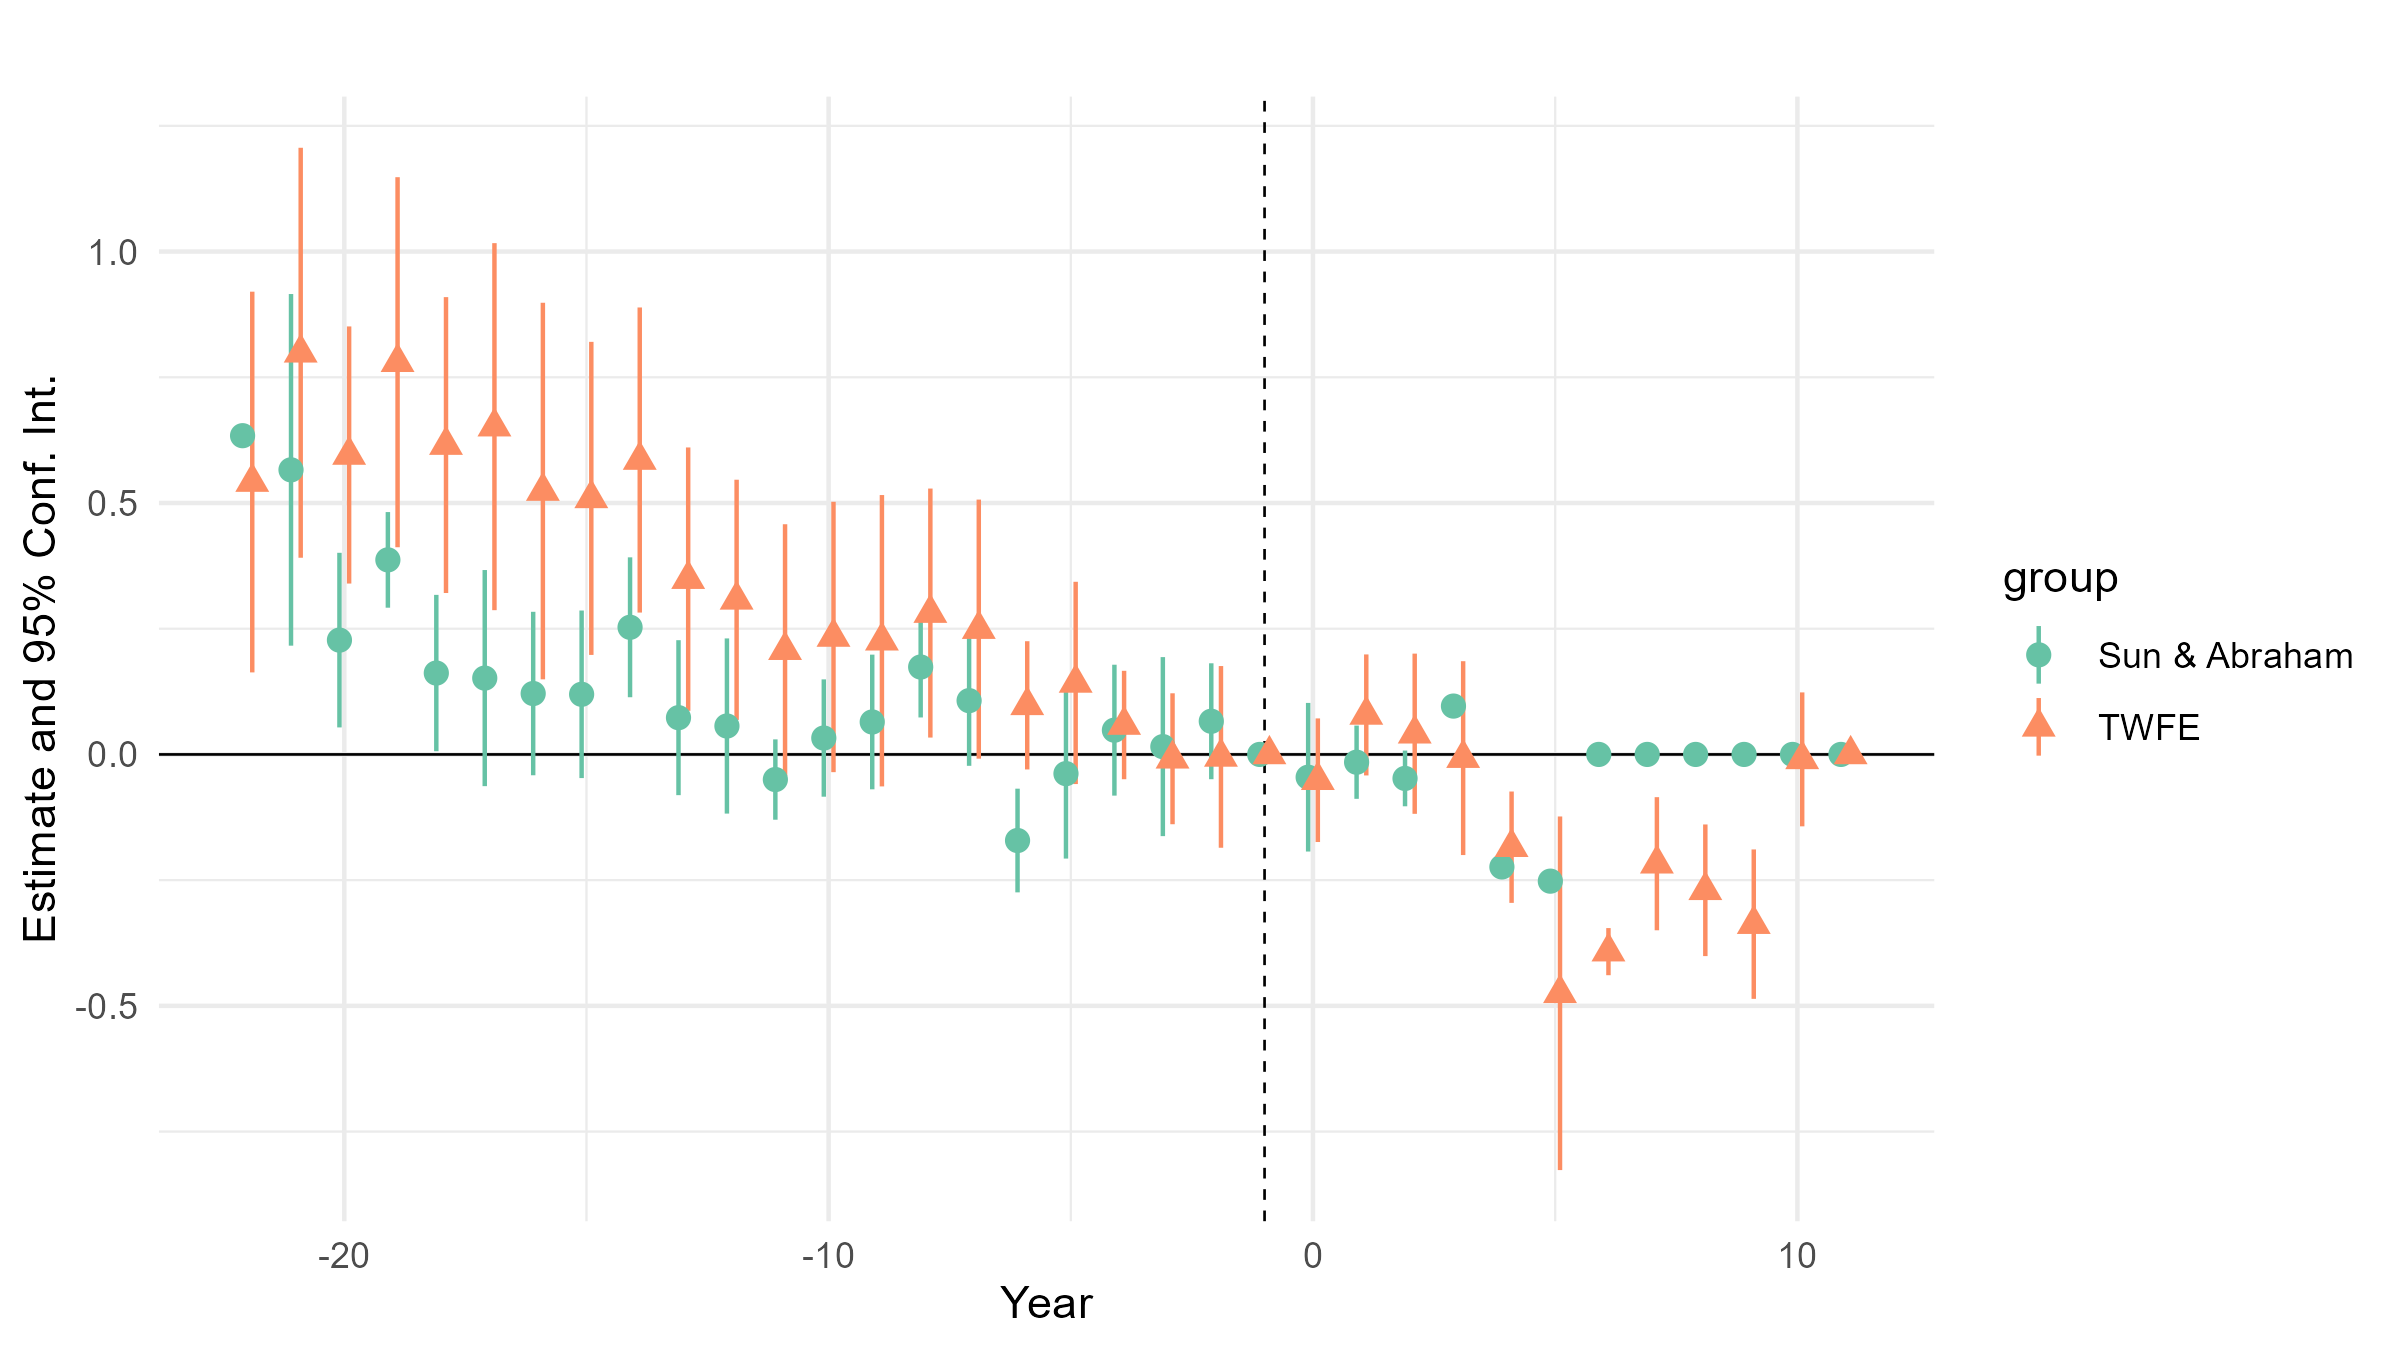
\includegraphics[width=.85\textwidth]{figures/figure1.png}
    \end{center}
    \caption{Treatment's effect on Murder}
    \label{fig:graph}
\end{figure}

\begin{figure}[H]
    \begin{center}
        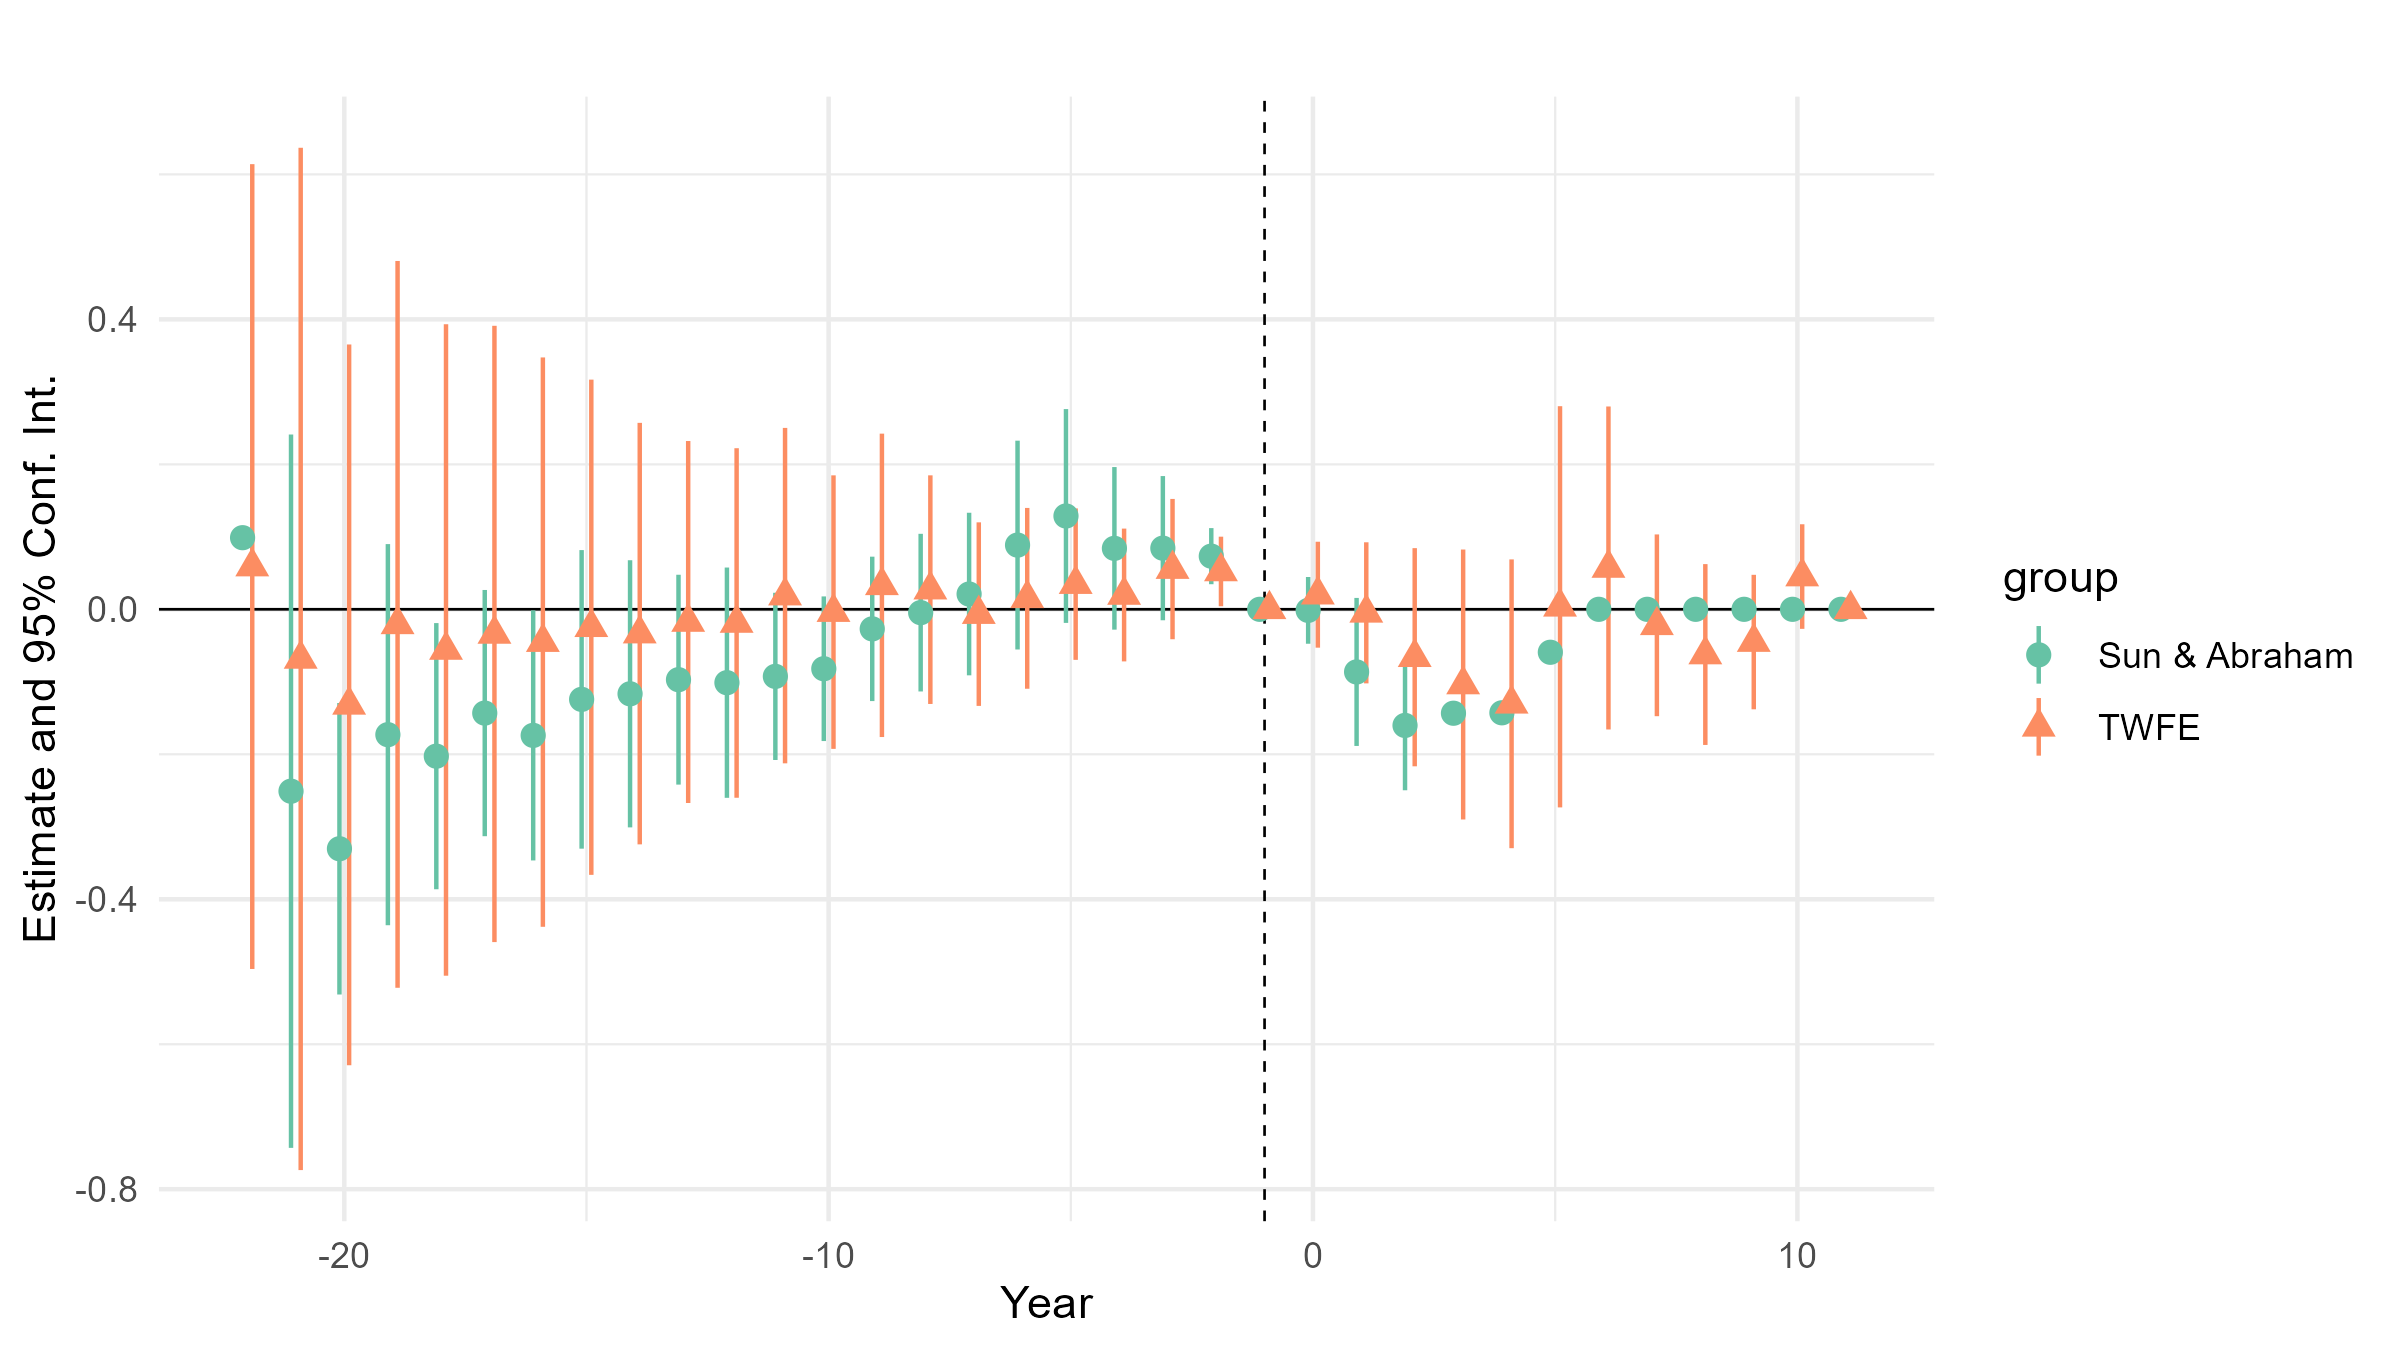
\includegraphics[width=.85\textwidth]{figures/figure2.png}
    \end{center}
    \caption{Treatment's effect on Rape}
    \label{fig:graph}
\end{figure}

\begin{figure}[H]
    \begin{center}
        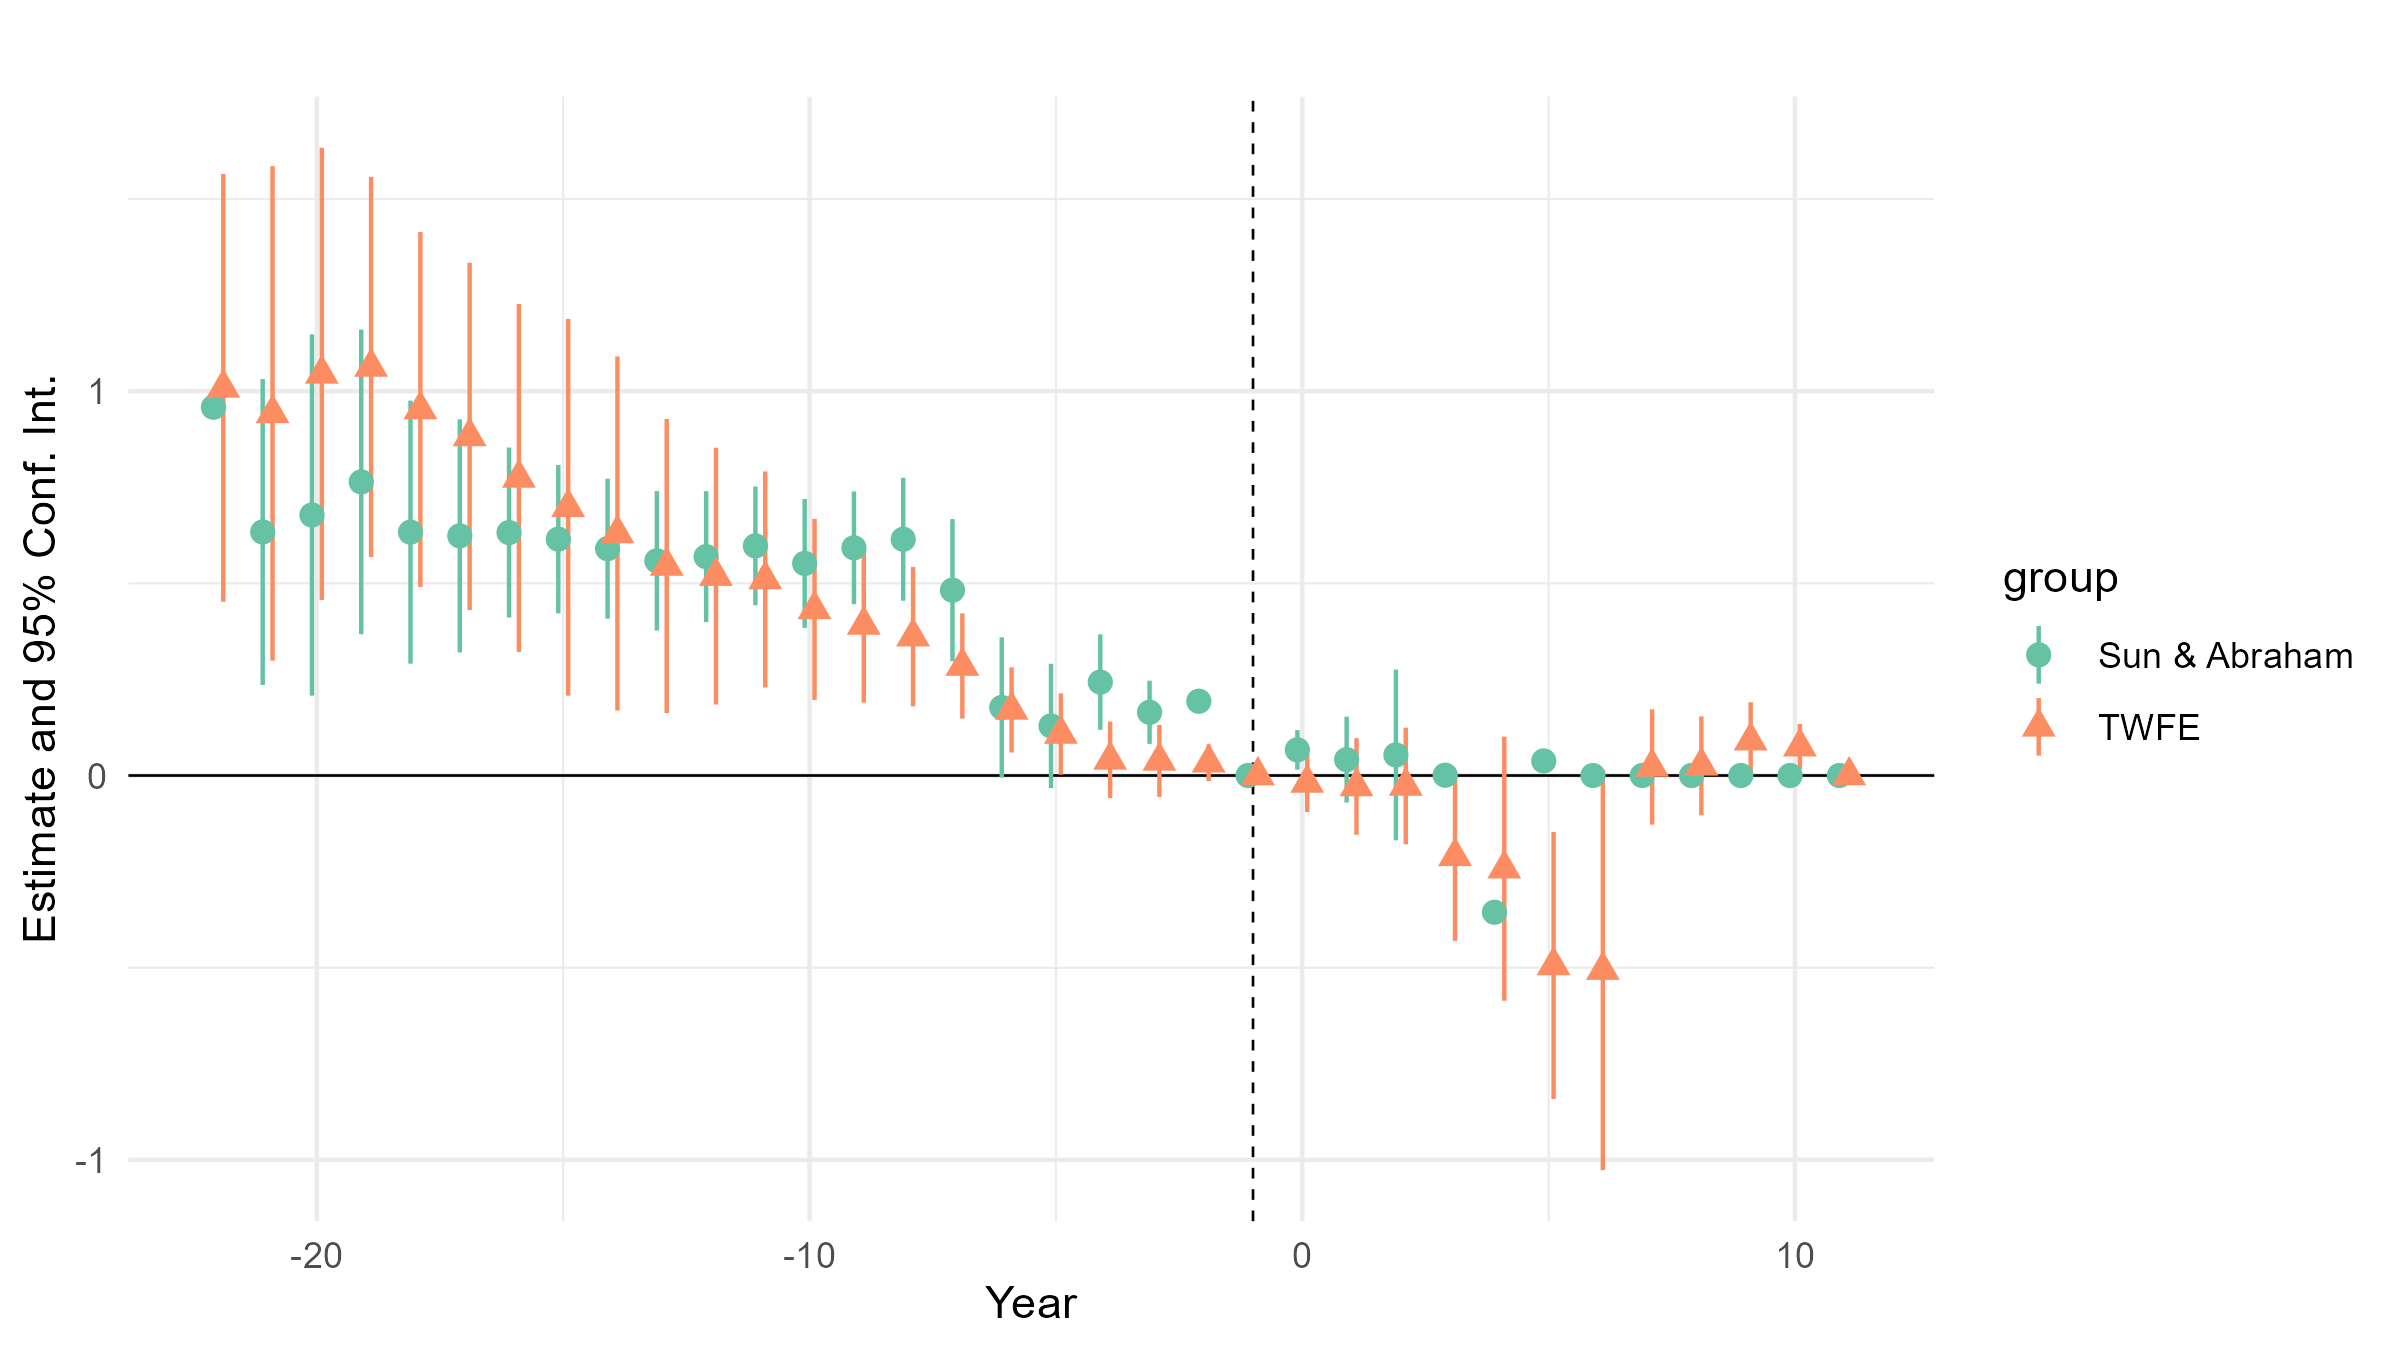
\includegraphics[width=.85\textwidth]{figures/figure3.png}
    \end{center}
    \caption{Treatment's effect on Aggravated Assault}
    \label{fig:graph}
\end{figure}

\begin{figure}[H]
    \begin{center}
        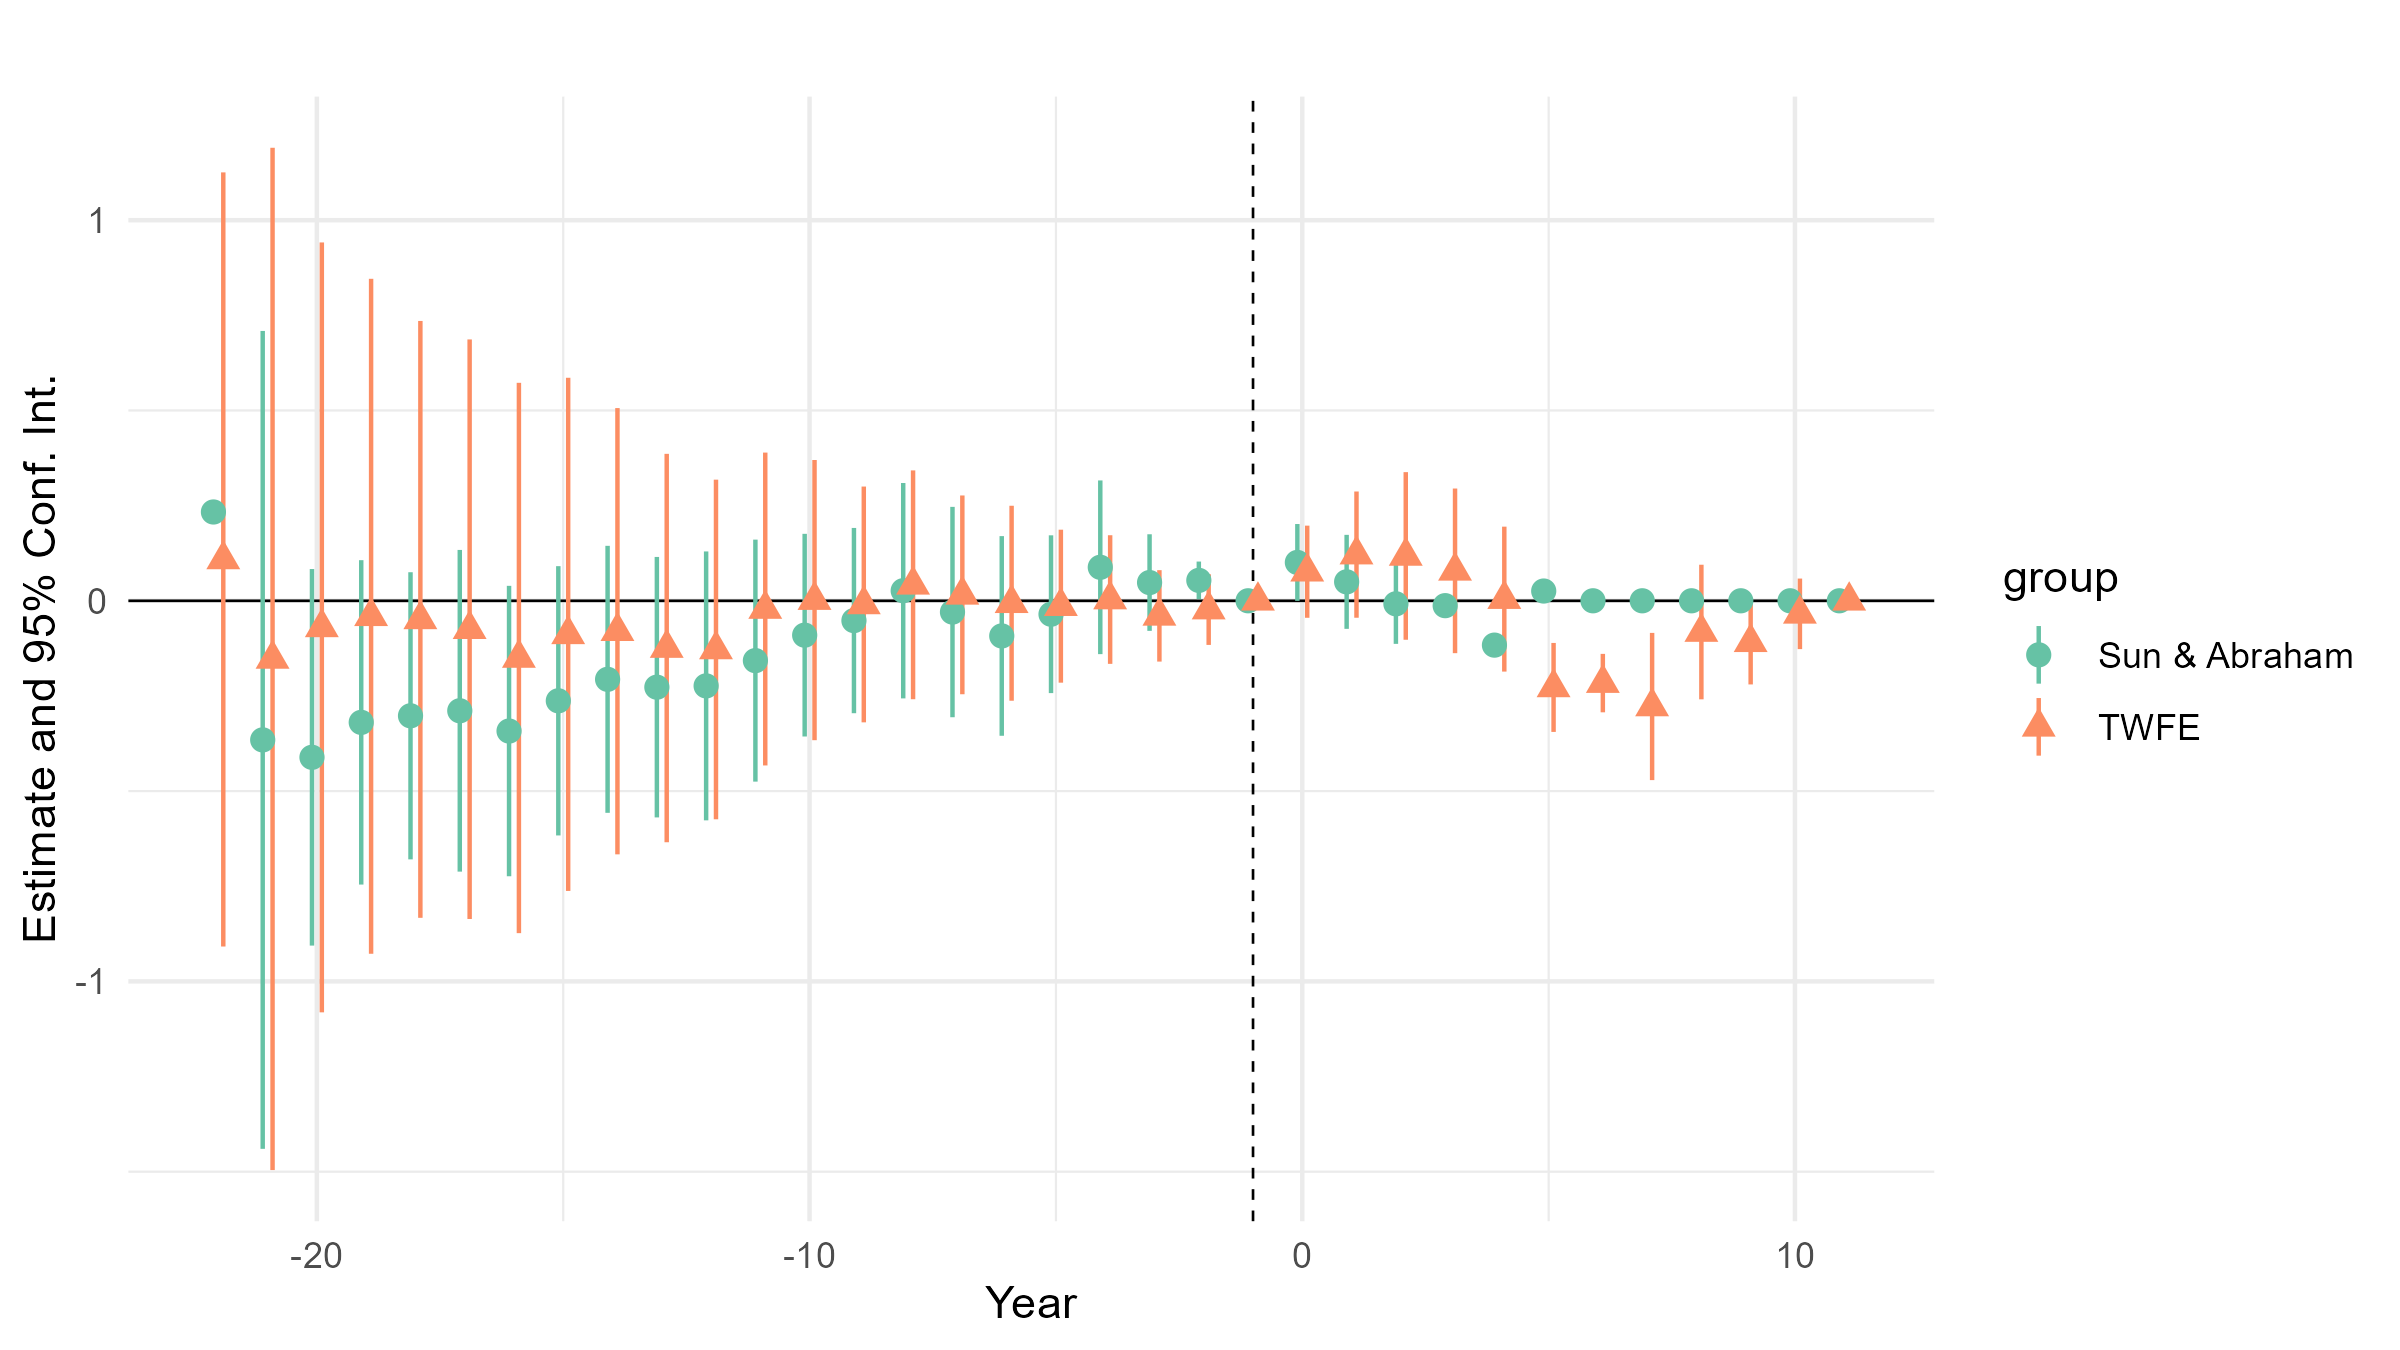
\includegraphics[width=.85\textwidth]{figures/figure4.png}
    \end{center}
    \caption{Treatment's effect on Robbery}
    \label{fig:graph}
\end{figure}

\begin{figure}[H]
    \begin{center}
        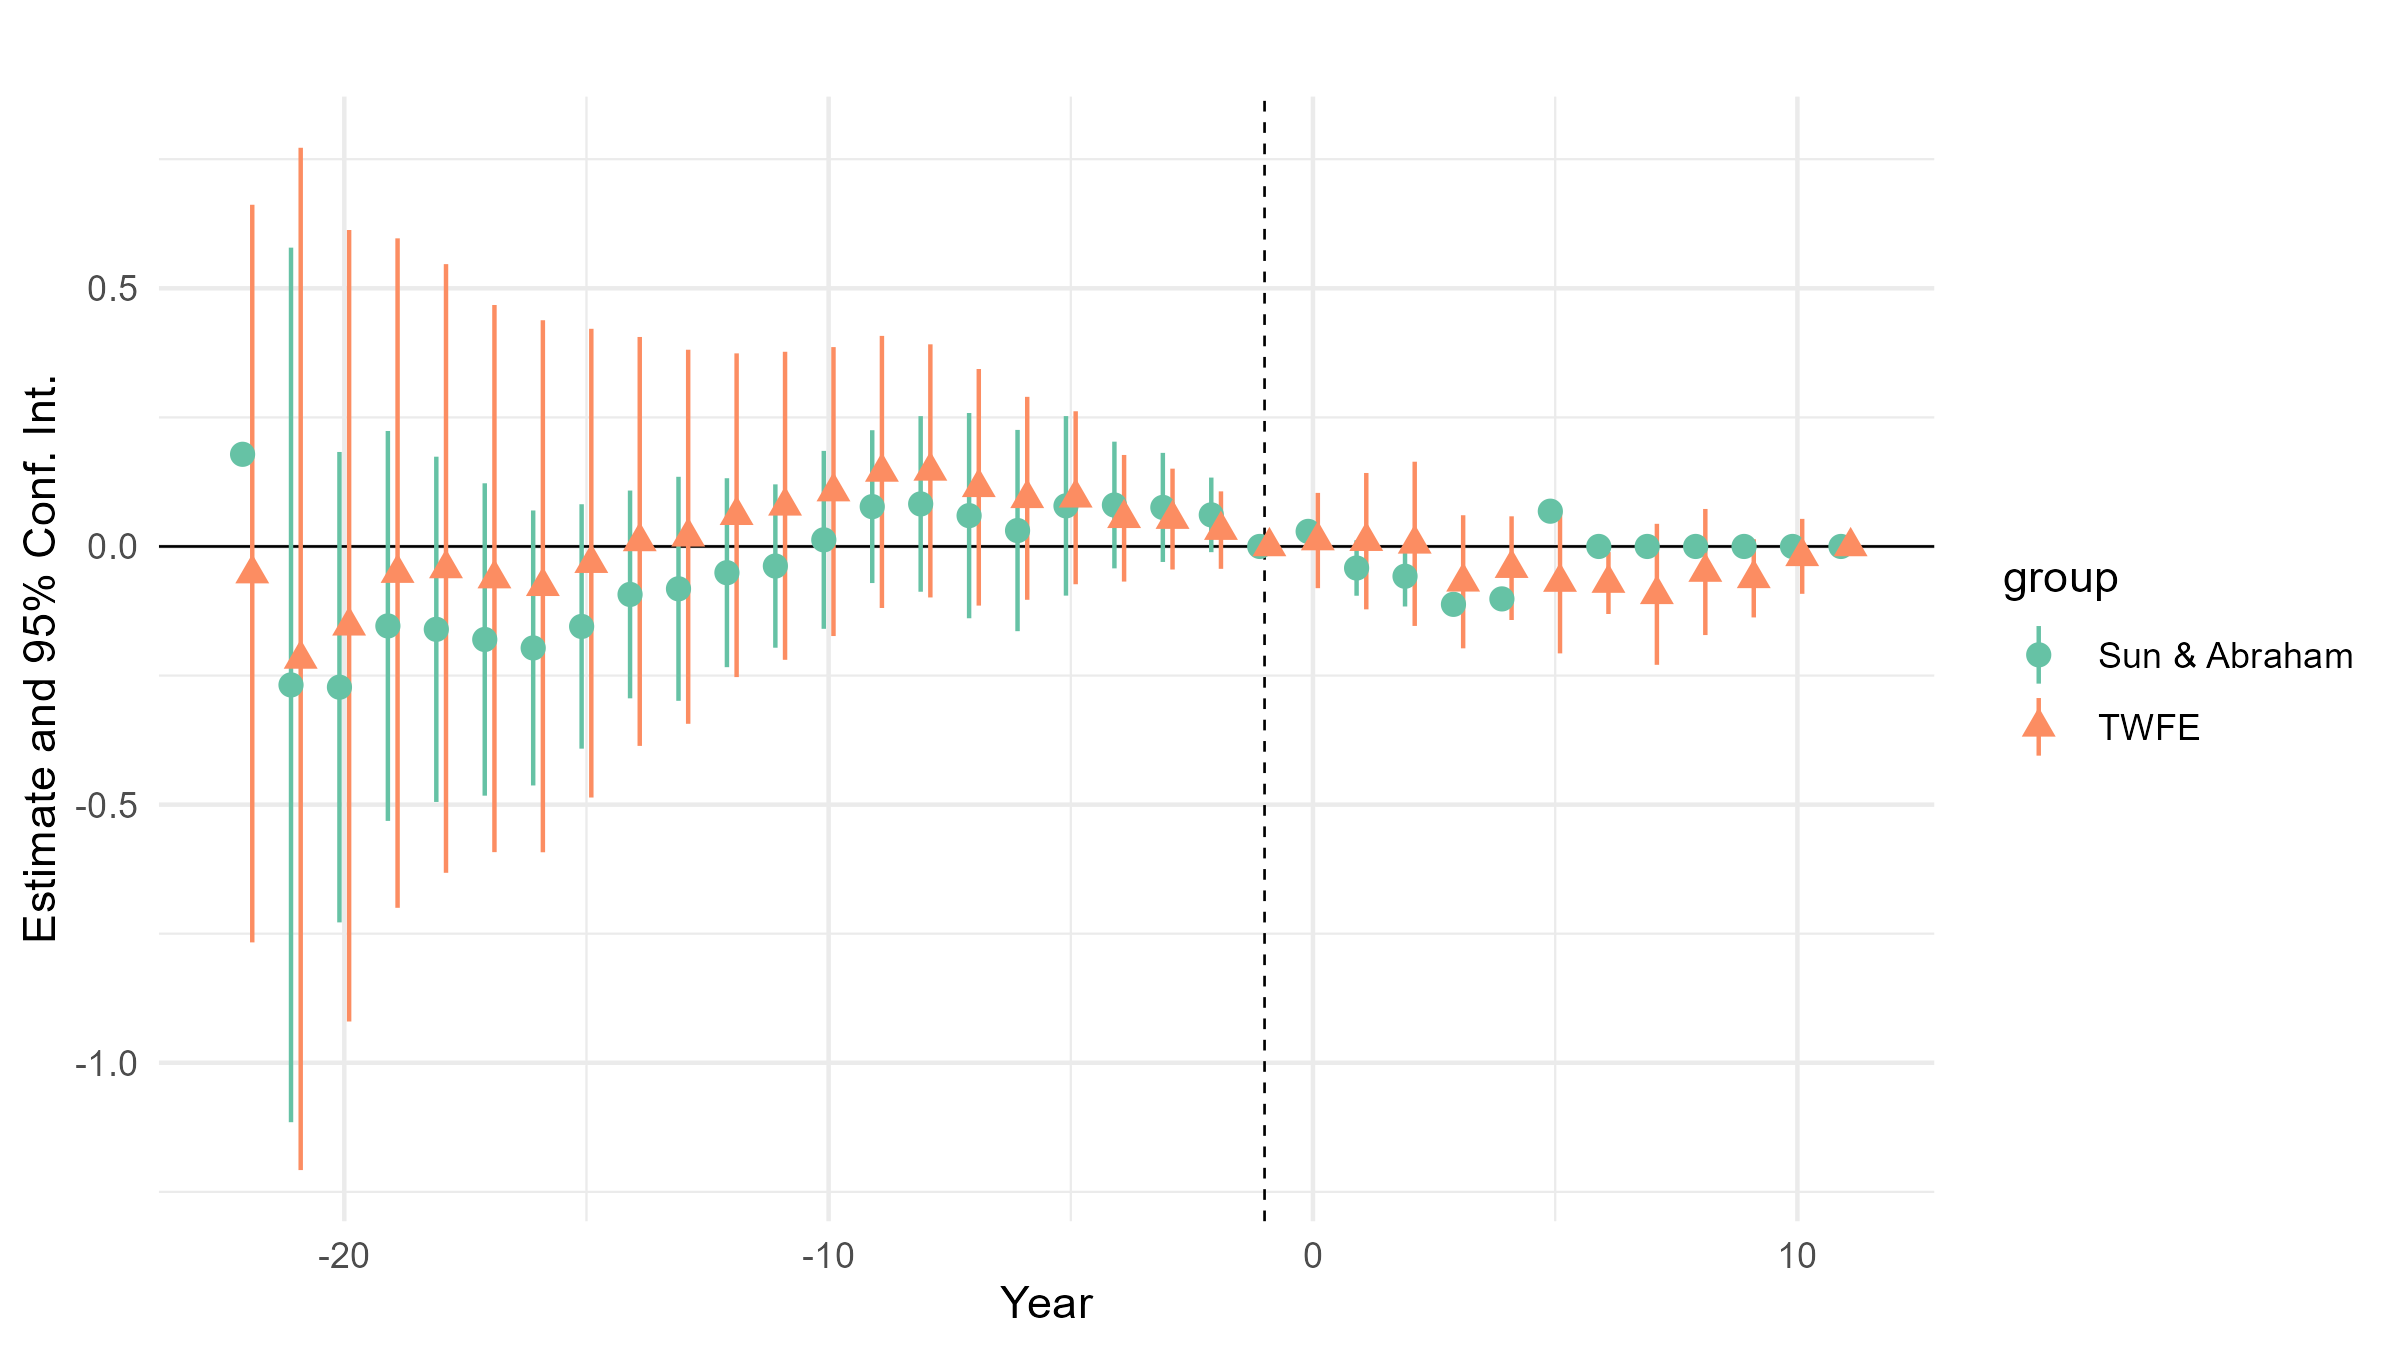
\includegraphics[width=.85\textwidth]{figures/figure5.png}
    \end{center}
    \caption{Treatment's effect on Burglary}
    \label{fig:graph}
\end{figure}

\begin{figure}[H]
    \begin{center}
        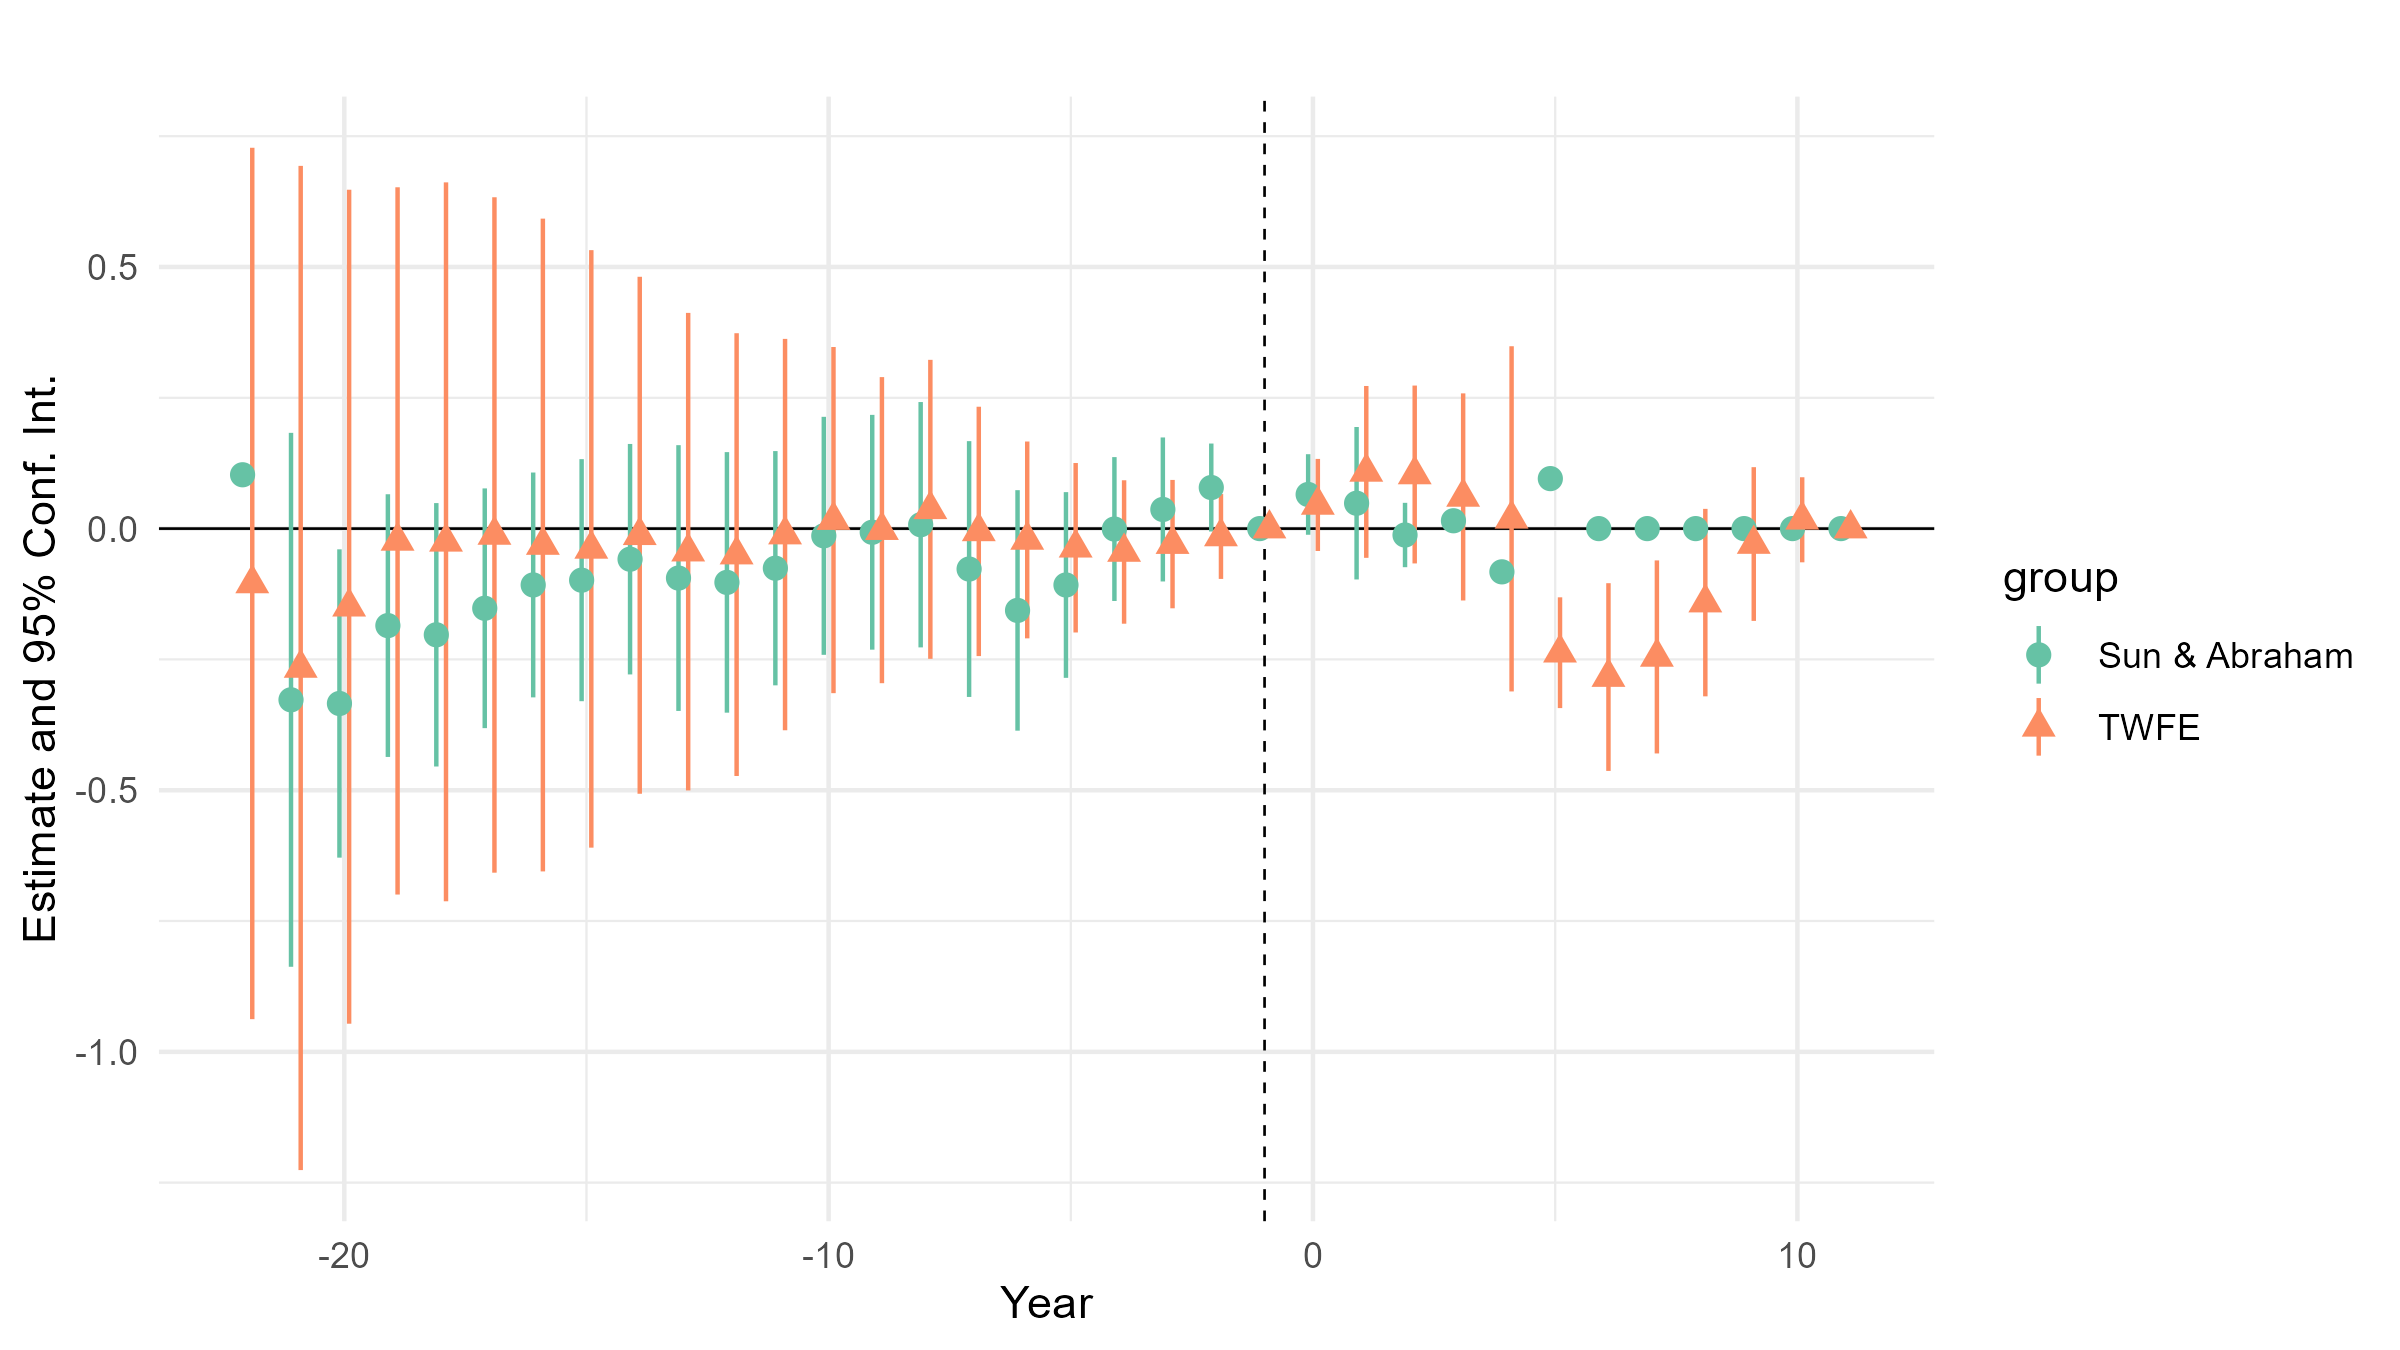
\includegraphics[width=.85\textwidth]{figures/figure6.png}
    \end{center}
    \caption{Treatment's effect on Auto Theft}
    \label{fig:graph}
\end{figure}

\begin{figure}[H]
    \begin{center}
        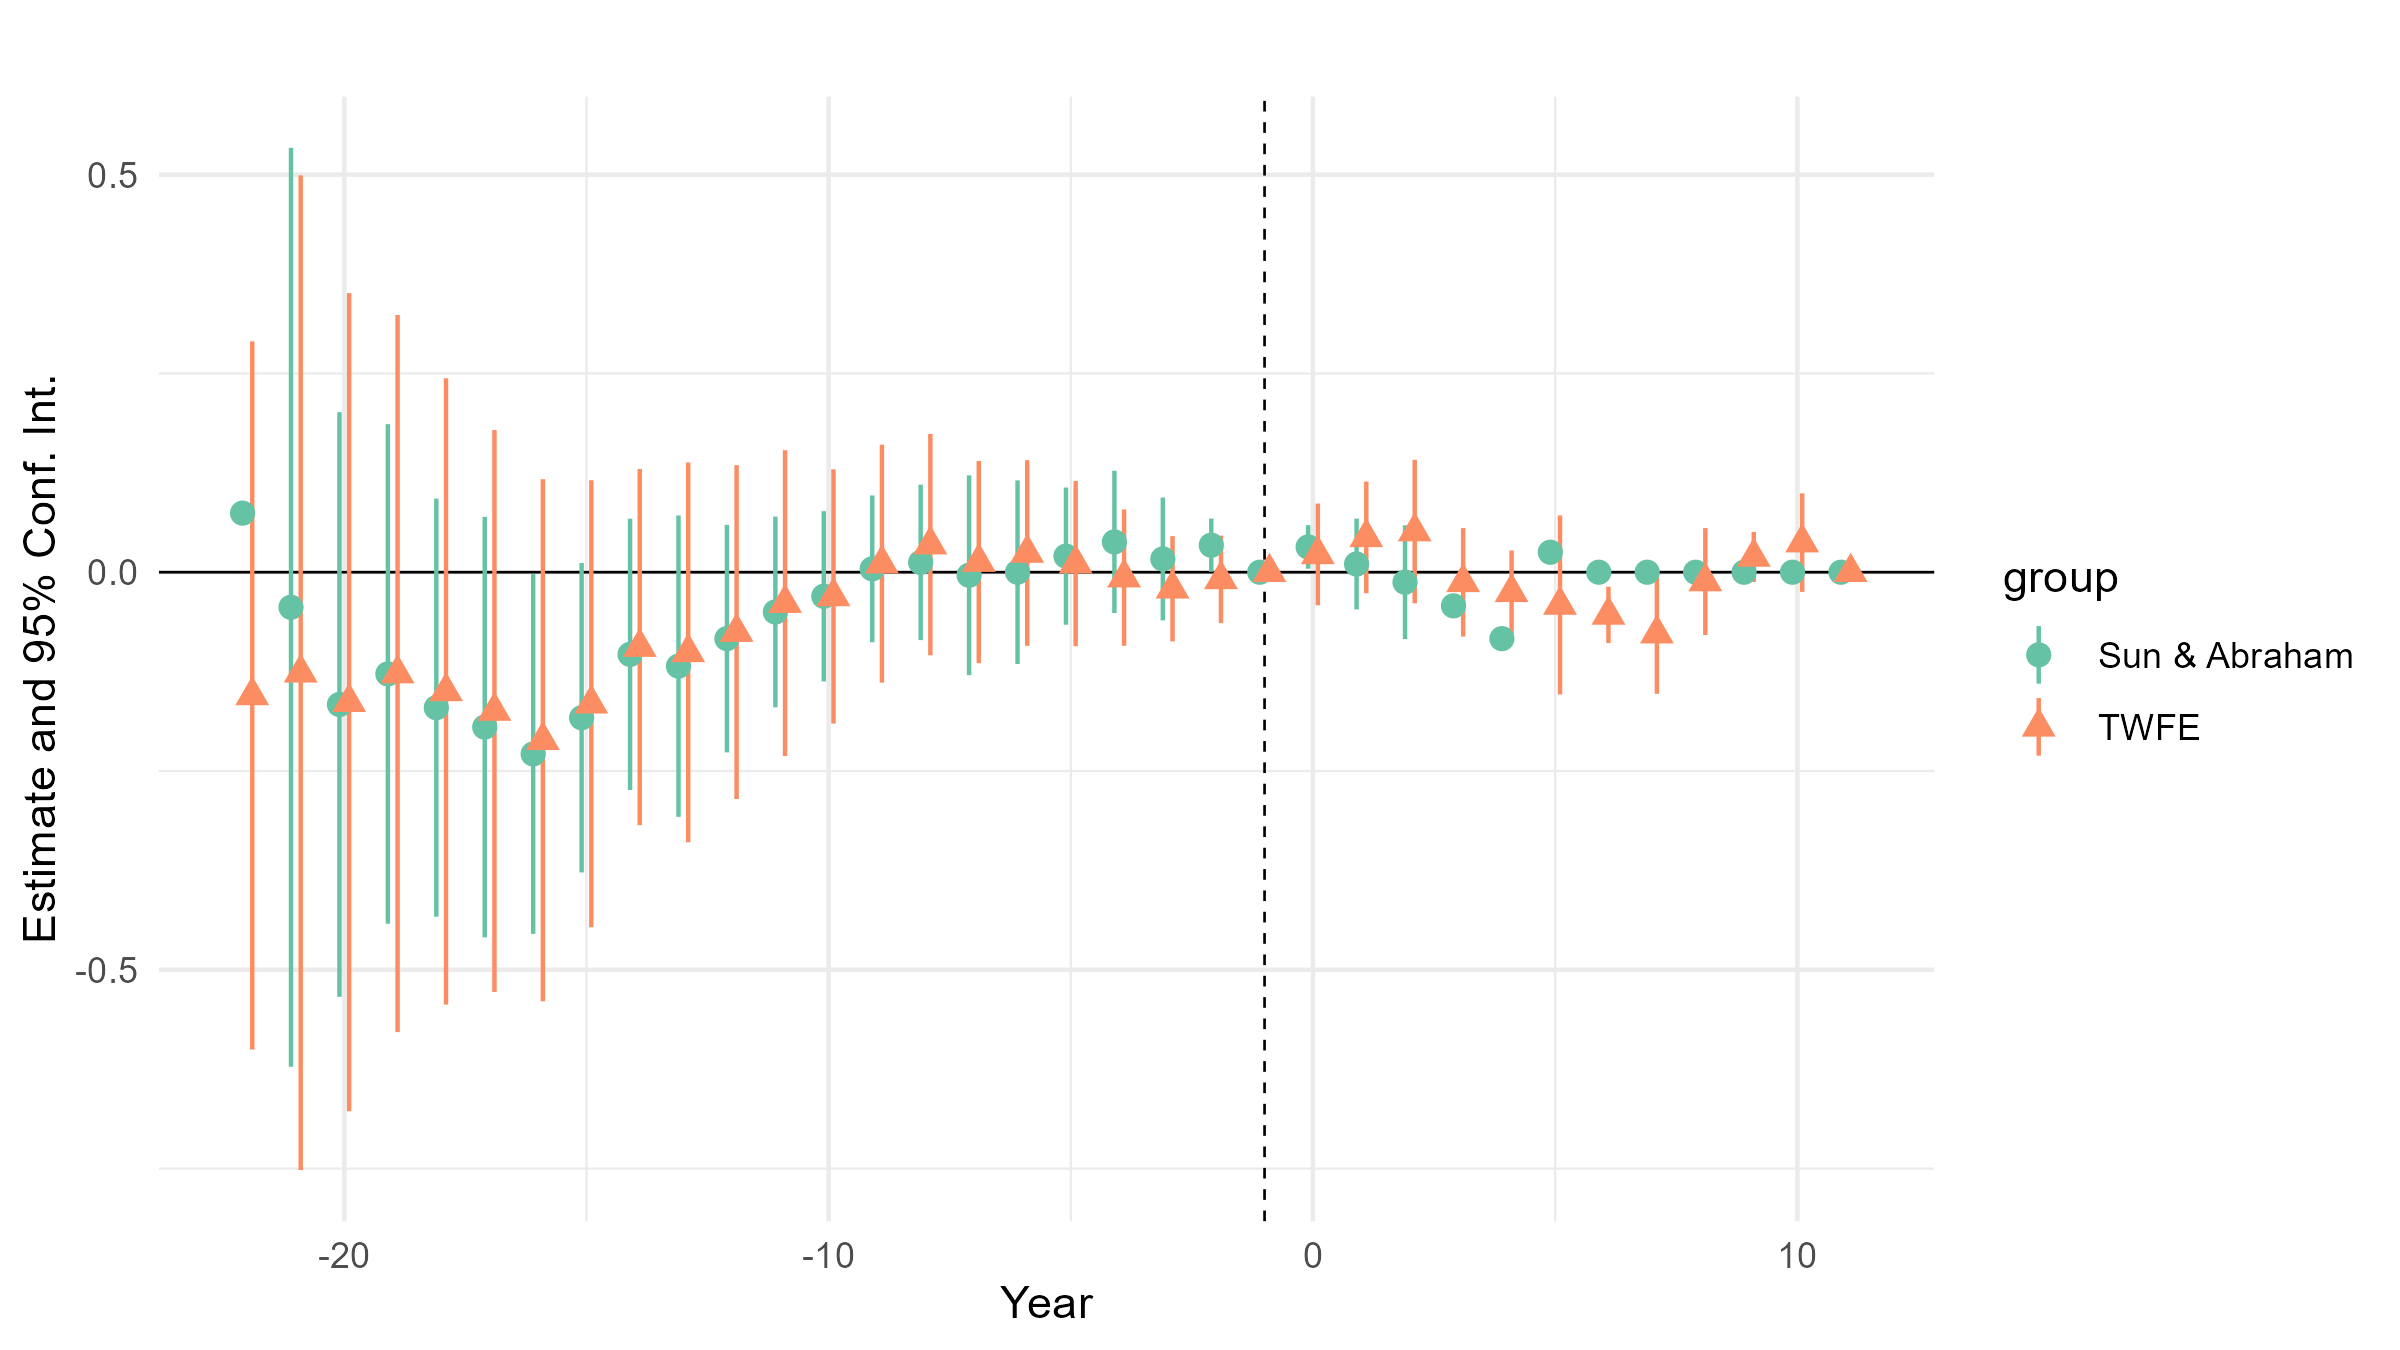
\includegraphics[width=.85\textwidth]{figures/figure7.png}
    \end{center}
    \caption{Treatment's effect on Larceny}
    \label{fig:graph}
\end{figure}

\end{document}